\section{连续函数}
\subsection{连续点}
\begin{definition}\label{definition:极限.函数在一点的连续性}
%@see: 《数学分析(上册)》(陈纪修) P88 定义3.2.1
%@see: 《高等数学(第六版 上册)》 P61 定义
设函数\(f\)在点\(x_0\)的某一邻域内有定义.
如果\[
	\lim_{x \to x_0} f(x) = f(x_0),
\]
那么就称“函数\(f\)在点\(x_0\)~\DefineConcept{连续}
(\(f\) is continuous at \(x_0\))”,
称“点\(x_0\)是函数\(f\)的\DefineConcept{连续点}(point of continuity)”.
\end{definition}

上述对函数连续的定义可以简化为:\[
	\text{\(f\)在点\(x_0\)连续}
	\iff
	(\forall\epsilon>0)
	(\exists\delta>0)
	(\forall x)
	[
		\abs{x - x_0} < \delta
		\implies
		\abs{f(x) - f(x_0)} < \epsilon
	].
\]

\begin{definition}
%@see: 《数学分析(上册)》(陈纪修) P89 定义3.2.3
如果函数\(f\)在点\(x_0\)的某一左邻域内有定义,
极限\(f(x_0^-) = \lim_{x \to x_0^-} f(x)\)存在,
且\[
	f(x_0^-) = f(x_0),
\]
则称“函数\(f(x)\)在点\(x_0\)~\DefineConcept{左连续}
(\(f\) is left-continuous at \(x_0\))”.
\end{definition}

\begin{definition}
%@see: 《数学分析(上册)》(陈纪修) P89 定义3.2.3
如果函数\(f\)在点\(x_0\)的某一右邻域内有定义,
极限\(f(x_0^+) = \lim_{x \to x_0^+} f(x)\)存在,
且\[
	f(x_0^+) = f(x_0),
\]
则称“函数\(f(x)\)在点\(x_0\)~\DefineConcept{右连续}
(\(f\) is right-continuous at \(x_0\))”.
\end{definition}

\subsection{连续区间}
\begin{definition}
%@see: 《数学分析(上册)》(陈纪修) P89 定义3.2.2
如果函数\(f\)满足\[
	(\forall x_0\in(a,b))
	[\text{\(f\)在点\(x_0\)连续}],
\]
那么称“函数\(f\)在开区间\((a,b)\)内连续”.
\end{definition}

\begin{definition}
%@see: 《数学分析(上册)》(陈纪修) P90 定义3.2.4
如果函数\(f\)不仅在开区间\((a,b)\)内连续,
还在点\(a\)处右连续,且在\(b\)处左连续,
那么称“函数\(f\)在闭区间\([a,b]\)上连续”.
\end{definition}

\begin{remark}
上述定义可以统一地表示为如下形式:
设函数\(f\)在某区间\(X\)上有定义.
如果\[
	(\forall x_0\in X)
	(\forall\epsilon>0)
	(\exists\delta>0)
	(\forall x\in X)
	[
		\abs{x-x_0}<\delta
		\implies
		\abs{f(x)-f(x_0)}<\epsilon
	],
\]
则称“函数\(f\)在区间\(X\)上连续”.
\end{remark}

\begin{example}
有理整函数\[
	P_n(x) = a_0 x^n + a_1 x^{n-1} + \dotsb + a_n
\]在\((-\infty,+\infty)\)上连续.
\end{example}

\begin{example}
有理分式函数\[
	F(x) = \frac{P_n(x)}{P_m(x)}
\]在其定义域\(\Set{ x\in\mathbb{R} \given P_m(x)\neq0 }\)上连续.
\end{example}

\begin{example}\label{example:极限.正弦函数在实数域上连续}
%@see: 《数学分析(上册)》(陈纪修) P90 例3.2.3
证明:函数\(f(x) = \sin x\)在\((-\infty,+\infty)\)上连续.
\begin{proof}
任取\(x_0\in(-\infty,+\infty)\).
由\hyperref[equation:函数.三角函数.和积互化公式12]{和积互化公式}有\[
	\abs{\sin x - \sin x_0}
	= 2 \abs{\cos\frac{x+x_0}2 \sin\frac{x-x_0}2}
	= 2 \abs{\cos\frac{x+x_0}2} \abs{\sin\frac{x-x_0}2}.
\]
因为\((\forall\alpha\in\mathbb{R})[\abs{\cos\alpha}\leq1]\),
所以\[
	\abs{\sin x - \sin x_0} \leq 2 \abs{\sin\frac{x-x_0}2}.
\]
又因为当\(\alpha=0\)时有\(0=\sin\alpha=\alpha\),
而当\(\alpha\neq0\)时有\(0\leq\abs{\sin\alpha}<\abs{\alpha}\),
所以\((\forall\alpha\in\mathbb{R})[\abs{\sin\alpha}\leq\abs{\alpha}]\),
于是\[
	\abs{\sin x - \sin x_0}
	\leq 2 \abs{\frac{x-x_0}2}
	= \abs{x-x_0}.
\]
对于\(\forall\epsilon>0\),
取\(\delta=\epsilon\),
当\(\abs{x-x_0}<\delta\)时,
就有\(\abs{\sin x-\sin x_0}<\epsilon\),
所以\(\sin x\)在\((-\infty,+\infty)\)上连续.
\end{proof}
\end{example}

类似地可以证明,函数\(f(x) = \cos x\)在区间\((-\infty,+\infty)\)内是连续的.

% \begin{example}
% %@see: 《数学分析(上册)》(陈纪修) P91 例3.2.4
% 证明:函数\(f(x) = a^x\ (a>0,a\neq1)\)在\((-\infty,+\infty)\)上连续.
% \begin{proof}
% 首先有\[
% 	(\forall x_0\in\mathbb{R})
% 	[a^x-a^{x_0} = a^{x_0}(a^{x-x_0}-1)].
% \]
% 因此,证\(\lim_{x\to x_0} a^x = a^{x_0}\)就归结为证\(\lim_{t\to0} a^t = 1\).
% \end{proof}
% \end{example}

\subsection{间断点}
设函数\(f(x)\)在点\(x_0\)的某去心邻域内有定义.
在此前提下,如果函数\(f(x)\)有下列三种情形之一:
\begin{enumerate}
	\item 在\(x=x_0\)没有定义;
	\item 虽在\(x=x_0\)有定义,
	但\(\lim_{x \to x_0} f(x)\)不存在;
	\item 虽在\(x=x_0\)有定义,
	且\(\lim_{x \to x_0} f(x)\)存在,
	但\(\lim_{x \to x_0} f(x) \neq f(x_0)\),
\end{enumerate}
则称“函数\(f(x)\)在点\(x_0\)不连续”,
称“点\(x_0\)是函数\(f(x)\)的\DefineConcept{不连续点}或\DefineConcept{间断点}(discontinuity)”.

如果\(\lim_{x \to x_0}f(x) = \infty\),
则称点\(x_0\)为函数的\DefineConcept{无穷间断点}.
如\cref{figure:极限.无穷间断点},
点\(x=0\)是函数\(y=\frac{1}{x}\)的无穷间断点.

\begin{figure}[ht]
	\centering
	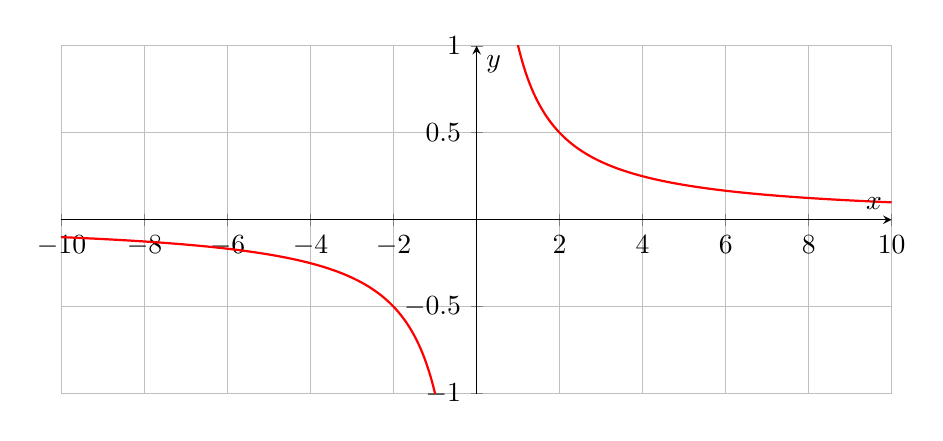
\begin{tikzpicture}
		\begin{axis}[
			xmin=-10,xmax=10,
			ymin=-1,ymax=1,
			grid=both,
			width=\textwidth,
			height=6cm,
			xlabel=$x$,
			ylabel=$y$,
			axis lines=middle,
		]
			\begin{scope}[samples=200,smooth,thick,red]
				\addplot[domain=-10:-.1]{1/x};
				\addplot[domain=+.1:+10]{1/x};
			\end{scope}
		\end{axis}
	\end{tikzpicture}
	\caption{}
	\label{figure:极限.无穷间断点}
\end{figure}

如果\(f(x)\)在点\(x_0\)的某一邻域是有界的,
但其左、右极限均不存在,则称点\(x_0\)为函数的\DefineConcept{振荡间断点}.
如\cref{figure:极限.振荡间断点},
点\(x=0\)是函数\(y=\sin\frac{1}{x}\)的振荡间断点.

\begin{figure}[ht]
	\centering
	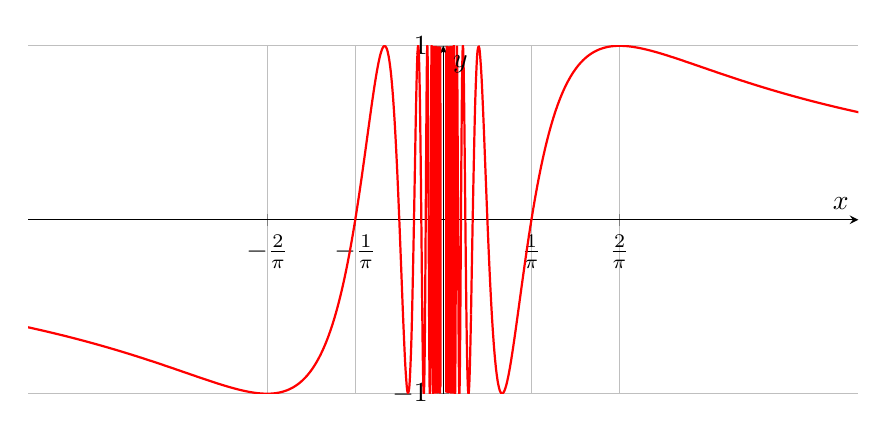
\begin{tikzpicture}
		\begin{axis}[
			xmin=-1.5,xmax=1.5,
			ymin=-1,ymax=1,
			grid=both,
			width=\textwidth,
			height=6cm,
			xlabel=$x$,
			ylabel=$y$,
			axis lines=middle,
			ytick={-1,1},
			xtick={-2/pi,-1/pi,1/pi,2/pi},
			xticklabels={$-\frac{2}{\pi}$,$-\frac{1}{\pi}$,$\frac{1}{\pi}$,$\frac{2}{\pi}$},
		]
			\begin{scope}[samples=200,smooth,thick,red]
				\addplot[domain=-5/pi:-.1]{sin(deg(1/x))};
				\addplot[domain=-.05:-.1]{sin(deg(1/x))};
				\addplot[domain=-.05:-.01]{sin(deg(1/x))};
				\addplot[domain=.05:.1]{sin(deg(1/x))};
				\addplot[domain=.05:.01]{sin(deg(1/x))};
				\addplot[domain=+.1:+5/pi]{sin(deg(1/x))};
			\end{scope}
		\end{axis}
	\end{tikzpicture}
	\caption{}
	\label{figure:极限.振荡间断点}
\end{figure}
